%% Included by 05-experiments.tex only when sections/family-numbers.tex exists (E02b done).
\begin{figure}[t]
  \centering
  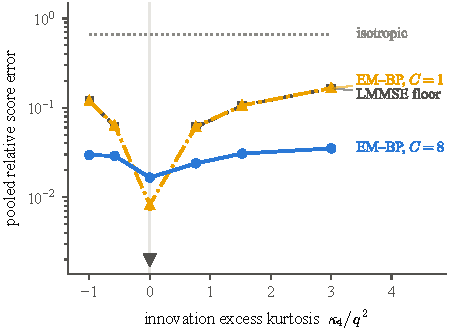
\includegraphics[width=\columnwidth]{fig_family.pdf}
  \caption{\textbf{Capacity buys exactly what the closure discards.} Pooled relative score
  error against the innovation's excess kurtosis for the generalised-Gaussian family at
  fixed $\corr$ and variance ($\nseq=\famSize$, $\famSeeds$ seeds, $\pm$ s.e.): the
  Gaussian-innovation kernel tracks the LMMSE floor, which is the exact price of
  second-order closure for each member; the mixture kernel tracks the exact score, and
  the two meet at the Gaussian member, where there is nothing beyond second order to
  learn.}
  \label{fig:family}
\end{figure}
Moving the innovation from Laplace (excess kurtosis $+3$) through the Gaussian to the
platykurtic end at fixed covariance (\cref{fig:family}), the LMMSE floor falls from
$\famLmmseBone$ to zero at $\beta=2$ and rises again to $\famLmmseBsix$; the
Gaussian-innovation kernel follows it, and the mixture kernel stays near
$\famEmeightBone$--$\famEmeightBsix$ throughout. The paired gain of $\ncomp=8$ over
$\ncomp=1$ is $\famDiffBone$ ($[\famDiffBonelo,\famDiffBonehi]$) at the Laplace end and
$\famDiffBtwo$ ($[\famDiffBtwolo,\famDiffBtwohi]$) at the Gaussian member, where the
two kernels are the same estimator up to sampling noise. Non-Gaussian capacity is worth
what \cref{thm:decay} says it is worth: the fourth-order structure the covariance twin
leaves behind.
